\section{Discussion}

Our study provides the first direct empirical test of the long-standing hypothesis that wind disrupts overwintering monarch butterfly clusters. For over three decades, conservation practice has operated under the assumption that wind speeds exceeding 2 m/s force butterflies to abandon their roosts, either by physically dislodging them or triggering behavioral departures \parencite{leongEvaluatingManagementCalifornia2016}. Our findings challenge this fundamental assumption and suggest a more complex relationship between monarchs and their overwintering environment.

\subsection{Evidence Against Wind Disruption}

The evidence against the wind disruption hypothesis emerges from multiple, independent lines of analysis. Most strikingly, every single observation period in our day-to-day analysis experienced maximum wind speeds exceeding the proposed 2 m/s threshold (range: 2.0--12.8 m/s), yet monarch clusters persisted throughout the 78-day study period. If the hypothesis were correct, we should have observed either mass departures when temperatures permitted flight or butterflies physically dislodged and littering the ground when too cold to fly, as described in the literature \parencite{leongRestorationOverwinteringGrove1999}. We observed neither.

Our bivariate analyses provide additional refutation. When we examined the simple relationship between wind speed and cluster size changes, we found essentially no correlation at either temporal scale (30-minute r = 0.04, n = 1,894; day-to-day r = 0.13, n = 96). These analyses tested the most basic prediction of the hypothesis that increasing wind speed should produce decreasing cluster sizes. The absence of this relationship across wind speeds ranging from calm conditions to six times the proposed threshold suggests that wind alone does not drive clustering decisions.

Statistical power was not a limitation. Our analysis achieved 87.5\% power to detect moderate effects and 98.5\% power for large effects. The wind disruption hypothesis predicts substantial, observable impacts, not subtle statistical signals. Our failure to detect these effects, despite adequate power and validated methodology that successfully identified other environmental signals, provides strong evidence against the hypothesis rather than merely absence of evidence.

\subsection{Thermoregulation as an Alternative Explanation}

While wind alone showed no disruptive effect, our models revealed that monarchs respond to environmental conditions through complex interactions, particularly between wind and solar exposure. This interaction emerged as the dominant environmental signal in both temporal analyses (30-minute F = 4.67, p < 0.001; day-to-day F = 4.10, p < 0.001), suggesting that the relationship between wind and monarch behavior depends critically on light conditions.

The wind-light interaction reveals three patterns. First, when butterflies experienced no direct sunlight, wind speed had no discernible effect on cluster dynamics across the entire observed range (0 to 12.4 m/s). Second, when butterflies were exposed to direct sun in calm conditions, cluster sizes consistently decreased. Third, at intermediate levels of both wind and sun exposure, cluster sizes increased rather than decreased.

One interpretation of these patterns invokes thermoregulation. When exposed to direct sun in calm conditions, butterflies may depart to avoid overheating, as \textcite{mastersMonarchButterflyDanaus1988} demonstrated that monarchs in direct sunlight can elevate body temperature above ambient conditions within minutes. The counterintuitive increases in cluster size at intermediate wind and sun levels could occur if wind provides convective cooling that counteracts solar heating. \textcite{mastersMonarchButterflyDanaus1988} showed that monarchs can dissipate heat while gliding using airflow across their bodies; environmental wind might provide similar cooling without the energetic cost of flight. Shaded butterflies experience no solar heat gain, so wind would provide no thermal benefit, potentially explaining the absence of wind effects in shade. However, other behavioral mechanisms could produce these same patterns.

Additional observations align with thermal management. Time since sunrise revealed strong diurnal patterns (30-minute F = 9.85, p < 0.001), with butterflies departing clusters in late morning and early afternoon, then reforming aggregations later in the day. This pattern persisted after controlling for temperature and sunlight, potentially reflecting endogenous circadian rhythms, though it also aligns with predictable daily thermal cycles. The midday dispersal may reflect routine activities such as patrolling flights or nectaring. Monarchs have been observed gliding during these dispersal periods, which could facilitate thermoregulatory cooling while accomplishing other essential behaviors. Our study could not follow individual butterflies once they departed cluster locations, so these activities remain speculative. Similar temporal patterns have been consistently documented at California overwintering sites \parencite{tuskesOverwinteringEcologyMonarch1978,chaplinEnergyReservesMetabolic1982}, and the Xerces Society's standardized monitoring protocols explicitly restrict counting to specific time windows to account for these diurnal movements \parencite{xercessocietyStepbyStepWesternMonarch2017}.

Our models explained 6.4\% of variance in 30-minute cluster changes and 39.7\% of variance in day-to-day roost fidelity. The environmental factors that did explain variance were predominantly thermal in nature: the wind-light interaction, direct sunlight exposure, and diurnal patterns of dispersal and aggregation. While substantial variation remains unexplained, the environmental signals we detected suggest thermal factors may play a more important role than wind avoidance in organizing clustering behavior. Without direct body temperature measurements under varying environmental conditions, thermoregulation remains one plausible interpretation among potentially others, and further research is needed to confirm the underlying mechanisms.

\subsection{Limitations and Context}

Several factors shape the interpretation of our findings. First, our data come from a single overwintering season (2023--2024) when monarch populations were relatively typical \parencite{xercessocietyWesternMonarchThanksgiving2025}. The following season saw near-complete absence of monarchs at our study sites, coinciding with the second-lowest overwintering population on record \parencite{xercessocietyWesternMonarchButterfly2025}. This dramatic population crash prevented temporal replication but underscores the urgency of understanding overwintering ecology with the data we have.

Second, our study observed relatively small clusters where butterflies maintained direct contact with eucalyptus substrates. The wind disruption hypothesis was developed during an era of massive aggregations containing hundreds of thousands of individuals, where many butterflies attached only to other butterflies in multi-layered formations \parencite{leongMicroenvironmentalFactorsAssociated1990,browerMonarchButterflyClusters2008}. If substrate attachment provides greater wind resistance than butterfly-to-butterfly attachment, wind might affect these different clustering configurations differently. The hypothesis may have been accurate for the extreme densities of past decades but less relevant to today's smaller populations.

Finally, our models explained relatively little variance overall (30-minute 6.4\%; day-to-day 39.7\%), reflecting both the complexity of butterfly behavior and our focus on testing specific hypotheses rather than comprehensively explaining movement patterns. However, the strong signals we did detect and our adequate statistical power give confidence in our main conclusion that wind alone does not disrupt monarch clusters as previously believed.

\subsection{Implications for Conservation}

Our findings suggest that strict adherence to wind protection thresholds may unnecessarily constrain habitat management. The absence of wind disruption despite frequent threshold exceedances indicates that suitable habitat within existing groves may be more extensive than currently recognized. Areas previously considered marginal due to wind exposure might support clusters if they provide appropriate thermal and light conditions.

However, we do not advocate abandoning tree planting. While wind protection may not directly prevent cluster disruption as previously thought, dense canopies provide other critical benefits: moderating temperature extremes, creating the dappled light patterns monarchs appear to prefer, and maintaining humidity levels that prevent desiccation. The fundamental practice of maintaining and restoring forest structure at overwintering sites remains sound, even if the mechanistic understanding requires updating.

Management focus might more productively shift toward understanding and maintaining thermal regimes within groves. As \textcite{sanieeHierarchyScaleInfluence2022} suggest, managing canopy structure to create appropriate light patterns and temperature gradients may be more important than achieving specific wind speed thresholds. This perspective aligns with our finding that the interaction between environmental factors, rather than single variables in isolation, shapes monarch clustering behavior.

\subsection{Future Research Directions}

Our findings open several important avenues for future research. While the wind-light interaction we observed suggests complex relationships between environmental factors and clustering behavior, the strong effect of light exposure itself points toward canopy structure as a potentially primary driver of habitat selection. This conclusion finds support in \textcite{sanieeHierarchyScaleInfluence2022}, who found that while temperature and humidity failed to support the microclimate hypothesis at aggregation locations, solar radiation was one of the few environmental factors that distinguished occupied sites from other grove locations. Similarly, \textcite{weissForestCanopyStructure1991} found that successful overwintering sites maintain consistent canopy openness around 20\%, while unsuccessful sites show greater variability (Figure~\ref{fig:weiss_canopy}). Combined with our findings, this suggests that predictable light patterns created by canopy structure may provide a stable, reliable environmental cue that monarchs can consistently locate and respond to year after year. Unlike weather conditions that fluctuate unpredictably, the spatial pattern of light created by canopy architecture remains relatively constant across seasons, offering a dependable signal for site selection. Monarchs possess sophisticated visual systems that enable sun compass navigation during migration \parencite{nguyenSunCompassNeurons2021,mouritsenVirtualMigrationTethered2002}, capabilities that would allow them to detect and respond to consistent light patterns within groves. Future research should prioritize characterizing canopy structure and the resulting light regimes at both occupied and unoccupied sites to determine whether specific light patterns predict roost site selection and fidelity.

\begin{figure}[h]
    \centering
    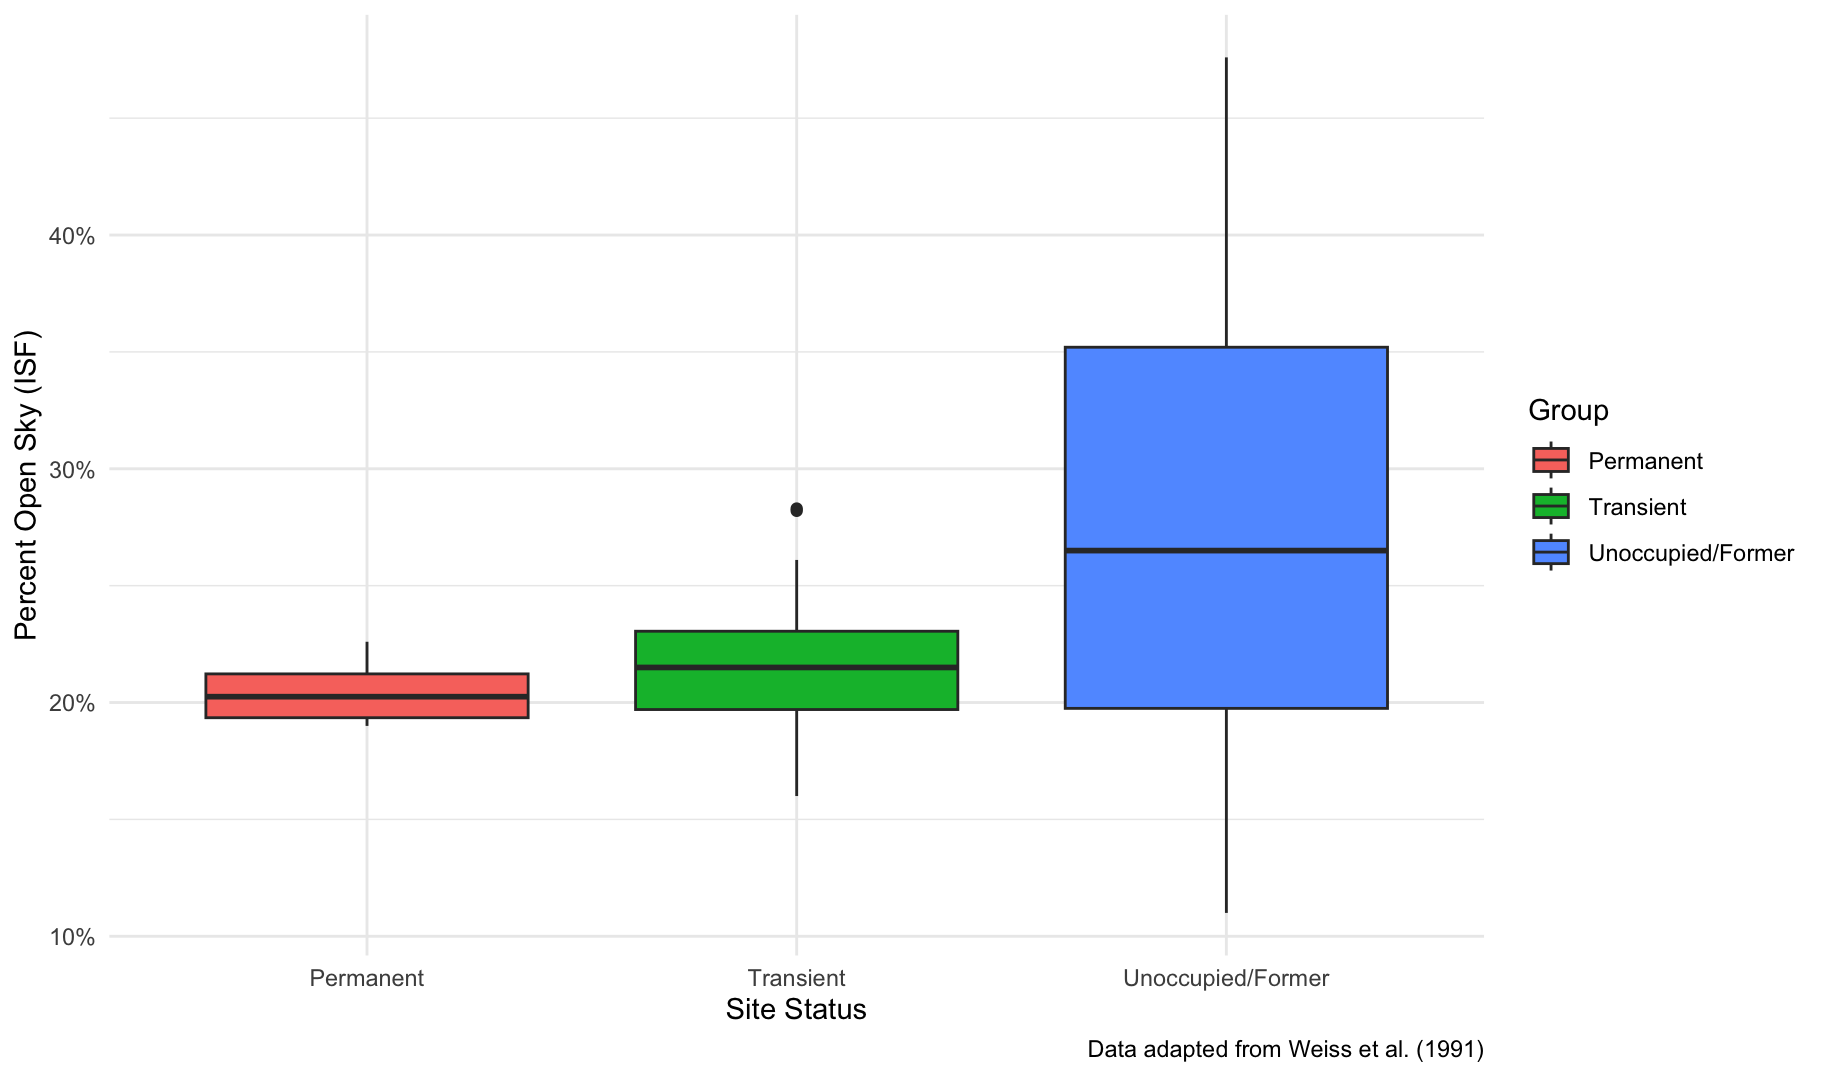
\includegraphics[width=0.8\textwidth]{figures/discussion/weiss_adapted_boxplot.png}
    \caption{Percent canopy openness (Indirect Site Factor) by occupancy status, adapted from Weiss et al. (1991). Permanent overwintering sites exhibit both a specific range of canopy openness (~20\%) and lower variance compared to transient and unoccupied/former sites.}
    \label{fig:weiss_canopy}
\end{figure}

Beyond environmental factors, social dynamics may explain additional variation in our models. The strong effect of previous butterfly count on subsequent changes suggests that monarchs do not distribute randomly within groves but rather exhibit overdispersed clustering patterns where the presence of butterflies attracts others. This positive feedback mechanism, where initial settlement increases the probability of others joining, could create self-reinforcing aggregation patterns independent of immediate environmental conditions \parencite{berdahlEmergentSensingComplex2013}.

Finally, testing these patterns across the broader overwintering range would establish their generality. Sites with different tree species, latitudes, and especially population densities could reveal whether wind responses vary with clustering configuration or if our findings represent fundamental aspects of monarch overwintering behavior.

\subsection{Conclusions}

Our direct test of the wind disruption hypothesis found no evidence that wind speeds above 2 m/s force monarchs to abandon their clusters. Every observation in our day-to-day analysis exceeded this threshold, yet clusters persisted. Bivariate analyses showed no relationship between wind and cluster changes. Model selection consistently identified other factors as more important. These multiple lines of evidence converge on a clear conclusion. Wind alone does not disrupt overwintering monarch butterflies as has been assumed for over three decades.

Instead, our results suggest that thermal factors may play a more important role in clustering dynamics than previously recognized. Monarchs responded strongly to direct sunlight and diurnal patterns, both factors that could influence body temperature. The unexpected wind-light interaction, where moderate wind combined with sun exposure sometimes increased cluster sizes, suggests that environmental conditions interact in complex ways that simple threshold-based management approaches cannot capture.

These findings arrive at a critical moment for monarch conservation. With western populations at historic lows, every assumption about habitat requirements deserves scrutiny. While questions remain about the precise mechanisms, our findings demonstrate that current management guidelines based on wind speed thresholds are not supported by empirical evidence. Moving forward, conservation efforts should prioritize maintaining existing overwintering groves while additional research clarifies what environmental factors monarchs select for when choosing roost sites. As we face the challenge of preserving overwintering habitat for a declining population, evidence-based understanding of monarch ecology becomes not just scientifically important, but essential for preserving the remarkable phenomenon of monarch migration in western North America.